\documentclass[10pt]{report}
\usepackage[utf8]{inputenc}
\usepackage{titlesec}
\usepackage{babel}
\usepackage{geometry}
\usepackage{graphicx}
\titleformat{\section}{\filright\normalfont\normalsize\bfseries\MakeUppercase}{\thesection.}{1em}{\normalsize}
\title{\textbf{\Huge Coursework 2: \protect\\Comparison of Data Fusion Methods for Estimating Orientation in 3-D Space Using Inertial Motion Sensors}}
\author{ \Large Adrian C. Nkadi - s1911455}
\date{}

 \titlespacing{\section}{0pt}{-15pt}{25.5pt}
 \titlespacing{name=\section, numberless}{0pt}{16pt}{15pt}
 \usepackage{color}   %May be necessary if you want to color links
\usepackage{hyperref}
\hypersetup{
    colorlinks,
    citecolor=black,
    filecolor=black,
    linkcolor=black,
    urlcolor=black
}
\usepackage[parfill]{parskip}
\begin{document}
\maketitle
\subsection*{1.Introduction}
The need to determine one’s orientation has been a problem that has existed for hundreds of years. The development of gyroscopes allowed for more accurate estimation of angular velocity. In contemporary times these measurements are combined with measurements against magnetic north and downward gravitational acceleration. These are taken from a single device called a Magnetic and Inertial Measurement Unit (MIMU) and their increasing availability [5] and ease of use are making their applicability more widespread. Indeed, The global Inertial Measurement Unit (IMU) market is projected to grow from \$16.41 billion in 2022 to \$28.37 billion by 2029 [20].

Orientation estimation is now used in vehicle travel, from autonomous vehicles to aircraft, ships, and military applications. It has also found use in virtual reality, as it is necessary to interface between the digital environment and the actions and movements of the human agent interaction with them. Even without the virtual environment, it has helped realise the full potential of inertial sensing in sporting and clinical applications. They also play a pivotal part in tracking human motion using multiple sensors and this data can even be used in animation to transpose human movements onto virtual avatars. \newline
\begin{figure}[!h]
  \caption{Several use cases of WIoT devices[1]}
  \centering
  \label{fig:mimuprev}
  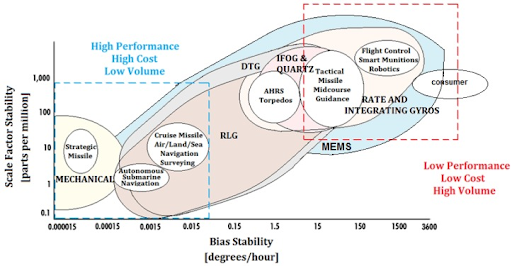
\includegraphics[]{mimuprevalance.png}
\end{figure}
\newline

With the increasing range and criticality of these estimation techniques especially for the prevalent low cost MIMUs (see Figure \ref{fig:mimuprev}), it is necessary to determine which techniques are best suited to what areas and devise stable baselines to compare the algorithms against each other.

In section 2, I will discuss some of the issues regarding state estimation that require the development of advanced algorithms to overcome. In section 3, I will describe the methods by which orientation can be represented and the benefits each bring for the same states. In section 4, I will then go on to talk about the measuring apparatus that is used to provide input for orientation estimation. In section 5 I describe the necessity of common baselines when comparing the methods and some propositions to achieve this. The limitations I highlight in sections 2 and 4 motivate the need for the sensor fusion algorithms (SFAs) that I describe and compare in section 6.

I will be comparing sensor fusion algorithms (SFAs) that use data from MIMUs to estimate pose and evaluate them as well as their applicability to different scenarios as defined by metrics relating to their computational expenditure.

Other methods of estimating orientation exist, for example, visual odometry methods that use camera data to determine position and orientation. However, this paper will only focus on MIMU-based methods.

A number of methods have been developed and most fall into three main categories. The first is the complementary filter family which uses low and high pass filters to obtain a corrected orientation signal. The second of which is the Kalman filter family which takes into account motion models and uncertainty to minimise error in the signal value. There is also a third variety called particle filters which use forecast and resampling approaches to obtain a best estimate of the true state of an object though this is not as popular as the other 2 [2].

\begin{figure}[!h]
  \caption{Classification of Sensor Fusion Algorithms Commonly used in Orientation Estimation[2]}
  \centering
  \label{fig:sfas}
  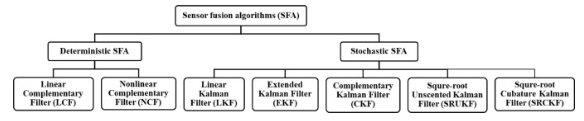
\includegraphics[width=1\textwidth]{sfas.PNG}
\end{figure}

\newpage

\subsection*{2. Estimation barriers}
The oldest and most basic method of determining orientation is using dead reckoning. Dead reckoning is simply taking the original orientation as well as the speed and direction of rotation along with the time after the last measurement to determine the new orientation. In most modern implementations that acceleration comes from the integration of a gyroscope's angular velocity reading. This method, however, introduces a number of errors.

The methods above are used for estimating the rotation relative to the initial rotation. However, there is uncertainty in that initial value itself most of the time. If a value far from the true orientation is estimated as the initial orientation then any method will determine its orientation as being incorrect even when they are close to the true value as its perceived base position moves relative to its own inertial frame.

Measurement noise is an issue in itself as every sensor has an associated bias and variance. Integration of velocity magnifies any error and bias that is present in the reading; this causes large errors that increase over time especially as gyroscopes drift over time.

SFAs leverage motion models to determine the equations to calculate the next position from the given values. However, even when the measurement noises are insignificant there will always be variables that are not accounted for. Temperature can, for example, affect the accuracy of motion models as gyroscopes behave differently as temperature changes. At higher angular speeds, gyroscopes are also susceptible to saturation error.

In order to determine relative orientation, you must have a baseline to compare against. Gravity is chosen as one of these baselines as its direction is always known and unchanging; if an object is aligned with gravity, that means it is travelling downwards. Likewise, for direction, a magnetometer is used to determine cardinal direction. Together, these two baselines can determine the object’s relative orientation on the x, y, and z axes. 

\newpage
\subsection*{3. Orientation Representation}
There are a number of methods to describe the orientation of an object in space. The difficulty comes in defining a notation that does not map multiple rotations to the same final position. One must also be careful to avoid singularities. The description of these parametrizations is particularly important as it is needed to evaluate and calibrate the sensor fusion models.

Euler rotation matrices are the standard method of describing rotation. However, this can result in singularities also known as Gimbal lock (see Figure \ref{fig:euler}. Quaternions are four dimension vectors that can also be used and they do not suffer from Gimbal lock but constrained estimation is required to avoid ambiguity as multiple Quaternion representations map to the same orientation. The defining equation of the Quaternion are shown in Figure \ref{fig:quat_equat} and a rotation can simply be written as $q_{GS}=(q_1,q_2,q_3,q_4)$. Direction cosine matrices can also be used to represent orientation as well as angular rate and they don’t suffer from singularities. However, integrating these matrices over time is very computationally expensive despite the simplicity of the equations. Furthermore, Quaternion normalisation introduces errors [6].

\begin{figure}[!h]
  \caption{Quaternion defining equation [10]}
  \centering
  \label{fig:quat_equat}
  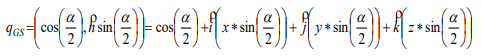
\includegraphics[width=1\textwidth]{quat_equat.PNG}
\end{figure}

\begin{figure}[!h]
  \caption{Gimbal lock formation in Euler Angles[10]}
  \label{fig:euler}
  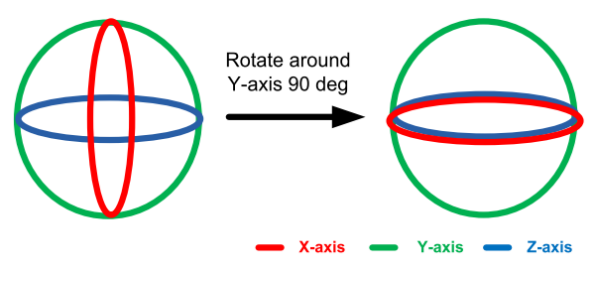
\includegraphics[width=0.8\textwidth]{eulerandgimbal.PNG}
\end{figure}

Multi-bin approaches can also be used where the possible rotations are defined as a set of overlapping discrete bins (see Figure \ref{fig:multibin}. The error in this case is defined using the confidence that the orientation falls in a given bin, taking into account the overlapping bin regions to judge that confidence. However, the application of this is relevant only to specific cases in vehicle travel.

\begin{figure}[!h]
  \caption{Multibin orientation method[11]}
  \label{fig:multibin}
  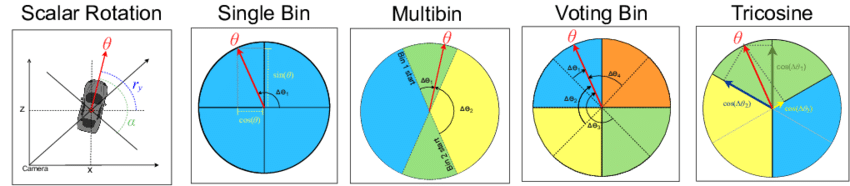
\includegraphics[width=1\textwidth]{multibin.PNG}
\end{figure}

\newpage

\subsection*{4. Measuring Apparatus}
MIMUs are the main providers of state information in modern times and they have grown small enough that they can be placed in an increased variety of situations increasing the applicability of both themselves and SFAs. These use cases extend to placement on human limbs for motion tracking.

Modern MIMUs are commonly composed of accelerometers that measure gravitational and motion-induced acceleration, magnetometers, and a tri-axial gyroscope. 

The accelerometer is used primarily to measure displacement but knowledge of the gravity component from when the MIMU is at rest enables the roll and pitch component of orientation to be determined. Furthermore, the orientation of the MIMU at any given time is necessary to calculate the displacement as gravity-induced acceleration must be discounted and orientation is needed to determine what direction gravity is acting in.

The magnetometer is used to determine the direction of the Earth’s magnetic north. From this yaw can be calculated. [7]

The most pertinent component of MIMUs to orientation estimation is the tri-axial gyroscope which measures angular velocity. Through the single integration of this gyroscope reading, relative orientation from the starting position can be readily determined. 

The accelerometer’s reliance on orientation to determine its own gravity component means that it cannot re-correct itself once in motion. The displacement the accelerometer is used to determine is also usually important. Furthermore, the accelerometer and magnetometers are both susceptible to external magnetic fields as they introduce biases to both sensors. In the case of the magnetometer, however, knowledge of true north isn’t so important as having a steady north reference point. The orientation determined by the gyroscope is derived by continuous integration but as this cannot be sampled at an infinitely high rate there is always a discrepancy between the true orientation and the estimated orientation and this discrepancy builds over time in a phenomenon called drift. This drift or angular random walk (ARW) makes long-term gyroscope-only orientation tracking unreliable [4] and its development from the double integration of acceleration magnifies it [1].
\newline
While it is possible to counteract the above effect, most low-cost MIMUs are not capable of effectively mitigating them, motivating the need for SFAs.

\subsection*{5. Baselining}
The issue with baselining lies not only in defining the metrics by which the SFAs are judged but also in defining the conditions and techniques used to calibrate them. Papers comparing methods usually have higher errors than those reported in papers originally proposing said methods by an order of up to one magnitude. As such multiple attempts have been made to standardise the conditions under which algorithms are compared. SFAs all rely on a set of gains to calibrate them for a given system. To calculate these gains in an effective manner, techniques such as particle swarm optimisation have been used to rigorously tune the SFAs before comparison. The study conducted by Nazarahari and Rouhani [2] conducted this tuning when running tests in 2 different phases. MIMUs also have widely varying errors and biases and perform differently at different temperatures and pressures among other factors [12]. As such, comparisons have been made using the same MIMU in the same temperature range and doing the same testing course. Another study conducted by Caruso et al [1] tested a select range of Kalman Filters and Complementary filters against 3 different MIMUs to verify their performance with different hardware.



\subsection*{6. Comparison Criteria}
When comparing SFAs their performance varies with the performance of their input unit. As such, multiple runs must always be made. As most measurement error with IMUs follows the white noise model [4], the mode, mean and median errors that multiple run aggregation would derive should amount to around the same value. This is due to the white noise Gaussian distribution.

The amount of computational resources the SFAs take is also paramount to most of their use cases as very little memory and computational power is usually allocated to orientation estimation as the main aim of the systems that employ them usually lies elsewhere. Furthermore, the execution speed of the algorithms needs to be high as well. This is related to the computational power required and is necessary for high-performance and fast-paced environments.

In many scenarios, the SFA may have one or all of its inputs disrupted, and in such situations, the MIMU be able to realign itself without explicit recalibration in order to remain reliable and robust. The convergence speed of the SFAs is also closely linked as many use cases require quick localisation in the order of 2 seconds or less (autonomous vehicles in many scenarios for example).

\newpage

\subsection*{7. Filter Comparison}
\subsubsection{7.1 Complementary Filters}
Complementary filters are a class of deterministic SFAs. They generally leverage low and high-pass filters to combine the fast-moving signals from a gyroscope with the slow-moving signals from accelerometers and magnetometers. At their most basic they use the equation shown in Figure \ref{fig:cf_equat} and alter the value of alpha to allocate confidence to state predictions from the accelerometer and gyroscope. This confidence value is affected by the sampling rate of the sensors as well as their error. an example of a full complementary framework is seen in figure \ref{fig:cfs}. Nonlinear variants also utilise the gating effect to discount acceleration after gravity removed is deemed too large in magnitude [9].

\begin{figure}[!h]
  \caption{Complimentary Filter Equation [10]}
  \centering
  \label{fig:cf_equat}
  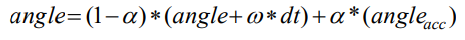
\includegraphics[width=1\textwidth]{cf_equat.PNG}
\end{figure}


\begin{figure}[!h]
  \caption{Framework of the Complimentary Filter Method [3]}
  \centering
  \label{fig:cfs}
  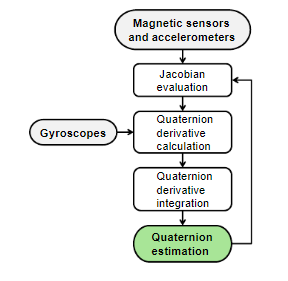
\includegraphics[width=0.4\textwidth]{cf.PNG}
\end{figure}

Extensions of this include the Mahony filter which compensates previous errors in angular velocity to obtain estimates of attitude which it recombines with results from the standard equation. Other extensions include using gradient descent algorithms for performance at low sampling rates, online magnetic distortion compensation and gyroscope bias. Madgwick [16] incorporates all of these but only enables the adjustment of fewer parameter allowing it to maintain low computation complexity. Justa2020[13] is a state-of-the-art method that uses prediction and correction steps to achieve a similar effect while keeping computational speed low. Other algorithms like Hua2014 use PID concepts like anti-integral windup to prevent the accumulation of errors.

In the second phase experiments of Nazahari's experiments [2], all but one of the complementary filters had median angle errors of “roughly 5° or less” and overall the difference between them was only slightly affected.

They tend to perform better than most at orientation estimation tasks involving sudden movements such as those common in the motions of human beings. It was these types of motions that were used for comparison in studies comparing SFAs in relation to human motion [1][3].


\subsubsection{7.2 Kalman Filters}
Kalman filters focus more on creating a process model that most accurately reflects the system it is operating in. They generally have models for measurement error and process error that they try to minimise in order to estimate the state without error. Similar to complementary filters, they can incorporate multiple estimates of state from different sensors but it combines the measurements based on how confident each input is in its prediction. The extent to which it trusts new measurements over its current data at any given time is encapsulated by the Kalman gain of the filter at that time.

Linear Kalman filters model processes in purely linear terms to determine transformation from state to state. In some filters, all the inputs are simultaneously processed in a single, connected set of equations to this effect. However, others such as Valenti 2016, or VAK as it is referred to in the study by Caruso et al [1], add robustness by separating the magnetometer-based transformations as they are typically less reliable.

Extended Kalman Filters (EKFs) use a probability distribution about a single point to represent the values it predicts after applying non-linear transformations to make those predictions. An example of a Kalman filter framework can be seen in figure \ref{fig:kfs}. In a variation of EKFs, Unscented Kalman Filters (UKFs) use multiple points to create the probability distributions.

The need for anatomical modelling of the process is clear [3], and this is especially important for Kalman filters. The Sabatini2006[15] reaps the benefit of such modelling. When standstill detection is used, Kalman Filters are also capable of resetting themselves such as when used for bicycles greatly boosting long term estimation [8].


\begin{figure}[!h]
  \caption{Framework of the Kalman Filter Method [3]}
  \centering
  \label{fig:kfs}
  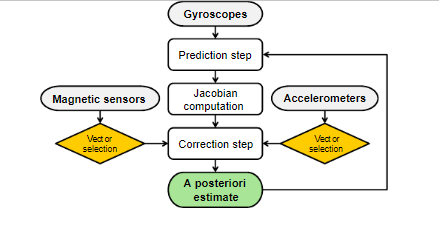
\includegraphics[width=0.6\textwidth]{kf.PNG}
\end{figure}

\newpage

\subsubsection{7.3 Particle Filters}
Particle filters work by predicting the probable next states given the distribution of current predictions on the state it has made and progressively discarding invalid predictions until it converges on a particle that it deems highly likely to be the true representation of the state. This is usually applied to estimate one’s position in an environment. These methods tend to be the most computationally expensive since they use simulation methods while other methods use direct simulation. No methods of this class were included in the aforementioned comparison papers and this is likely because of the poorer performance they generally have even at a high computational cost. 

\newpage
\subsubsection*{7.4 Cross Comparison}
Importantly, all SFAs compared using the particle swarm tuning method exhibited errors between 3.8 degrees and 7.1 degrees. As such, there is no statistically clear ranking based on accuracy alone based on those results. Even in figure \ref{fig:time}, where SF is an EKF and INT is dead reckoning, the 2 SFAs show little difference besides Kalman filters slight ability to re-correct themselves over time. This highlights how the context of application usually takes precedence and the auxiliary traits and functions of the SFAs should instead come to the fore when a decision on selection is to be made.

\begin{figure}[!h]
  \caption{Development of Heading and Attitude Errors over time [3]}
  \centering
  \label{fig:time}
  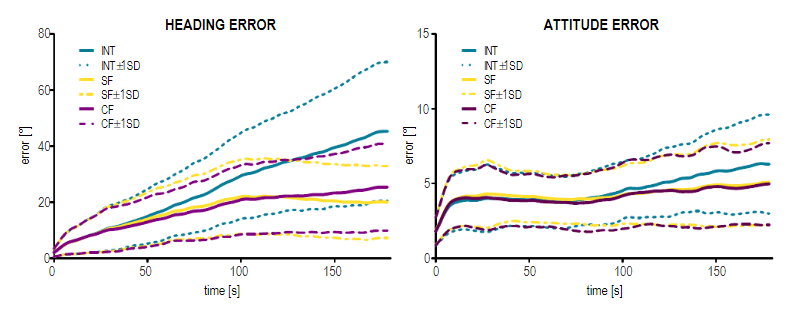
\includegraphics[width=1\textwidth]{compvstime.PNG}
\end{figure}


Complementary filters are generally seen to be the fastest method of sensor fusion, and the data shown in figure \ref{fig:exec} supports this. In neuroprosthetics systems where near real-time feedback is needed, this speed advantage becomes pivotal. It should also be noted that when optimising for computational speed, the accuracy of estimation usually is compromised.

\begin{figure}[!h]
  \caption{Comparison of error in manual routine (basic human motion tasks) and locomotion (high intensity activities) [1]}
  \centering
  \label{fig:locom}
  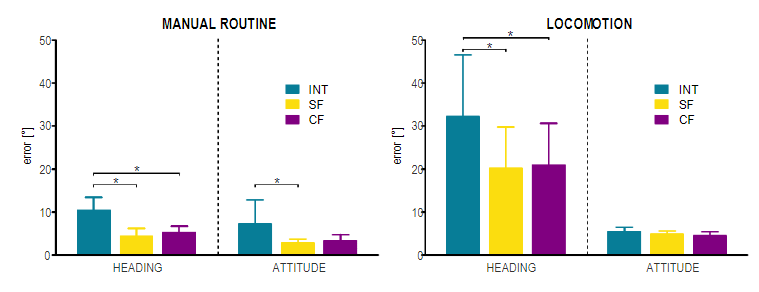
\includegraphics[width=0.8\textwidth]{routinevslocomotion.PNG}
\end{figure}

\newpage

\begin{figure}[!h]
  \caption{Execution times for10 SFAs- VAK,GUO, MKD, SAB and LIG are KFs and MAH, MAD, VAC, SEL and MCF are CFs [1]}
  \centering
  \label{fig:exec}
  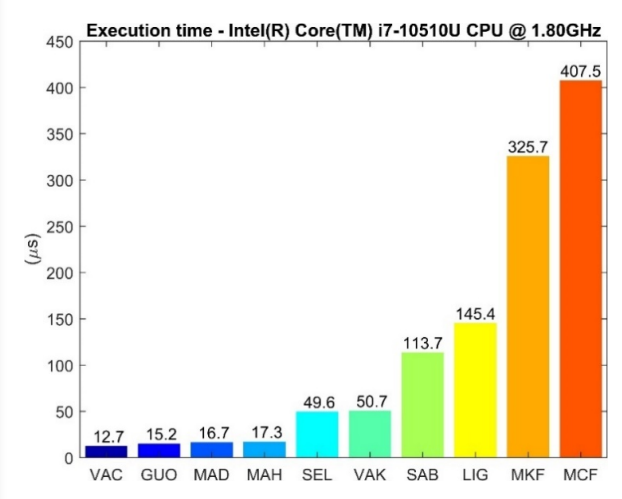
\includegraphics[width=0.7\textwidth]{exec.png}
\end{figure}

SFAs that were optimised based on quaternions were also shown to be hampered by the computational efficiency of quaternions. The quaternion library used by MATLAB for example was seen to be the limiting factor for the Valenti 2015 VAC implementation.

A large number of parameters does not guarantee better accuracy. In the standardised test environment, differences in accuracy can be put down to the increased difficulty that tuning more parameters causes even though they are more capable of modelling the sources of error in the system they are present in.

Saturation error causes increased error in both methods as per figure \ref{fig:locom} but while saturation error is present at high rotational speeds, high linear velocities are also shown to cause an error. This is because at higher velocities the estimate of gravity is less reliable. The direction of gravity is used by almost all methods to compensate for the effects of drift and the less reliable gravity direction information makes such compensation detrimental. The filters that do attempt to reject acceleration information at high magnitudes show unstable behavior near the thresholds that it rejects the information.





\subsection*{8. Conclusion}
It is evident that all the algorithms listed can perform to an acceptable standard for most cases so long as they are rigorously tuned and as such, it is that tuning that is the limiting factor. Furthermore, many algorithms operate differently under different scenarios

For most time-sensitive scenarios, the Hua2014[14] or Justa2020[13] algorithms would appear to be the preferred choices and this is highlighted by \ref{fig:fullcomp}. However, in environments where computational power isn’t as limited, the algorithm that showed the best performance was Sabatini's also further supported by \ref{fig:fullcomp}. This is underlined by the fact that an error of almost 72.8 with default parameters can be brought down to 2.5. Better tuning methods should be sought out to improve performance as well as algorithm development.

When high computational power is available, Kalman Filters do still provide benefits as at high speeds, Kalman Filters, such as Sabatini's (LIG in Caruso et al [1]), were capable of keeping error within range of what most other algorithms could do at low speeds (See Figure \ref{fig:inputcomp}). Generally, UKFs outperform EKFs in non-linear state estimation which most problems involve but EKFs have superior efficiency and stability [17]. LKFs fail to outperform either although Renaudin2014[19] comes close and is indeed the best in its class as per  \ref{fig:fullcomp}. However, they all outperform particle filters which despite their high computational cost are not as well suited to isolated state estimation but have excellent mapping capabilities [18].

All in all, these algorithms all help mitigate barriers to orientation estimation, vastly outperforming dead reckoning (See Figures \ref{fig:time} and \ref{fig:locom}).
\newpage
\begin{figure}[!h]
  \caption{ Statistical comparison of the root-mean-square (RMS) of the quaternion angle difference (QAD) among sensor fusion algorithms (SFAs) in one family for all testing data in Phase I and Phase II after gyroscope static bias removal. Significantly (p < 0.05) lower RMS(QAD), i.e. higher accuracy, for an SFA in a row compared to the ones in columns are identified with † for Phase I and with and ‡ for Phase II. * shows SFAs from each family with the lowest maximum error. The last column (score) shows the number of times an SFA significantly outperformed other SFAs in its family for Phase I and Phase II cumulatively. [2]}
  \centering
  \label{fig:fullcomp}
  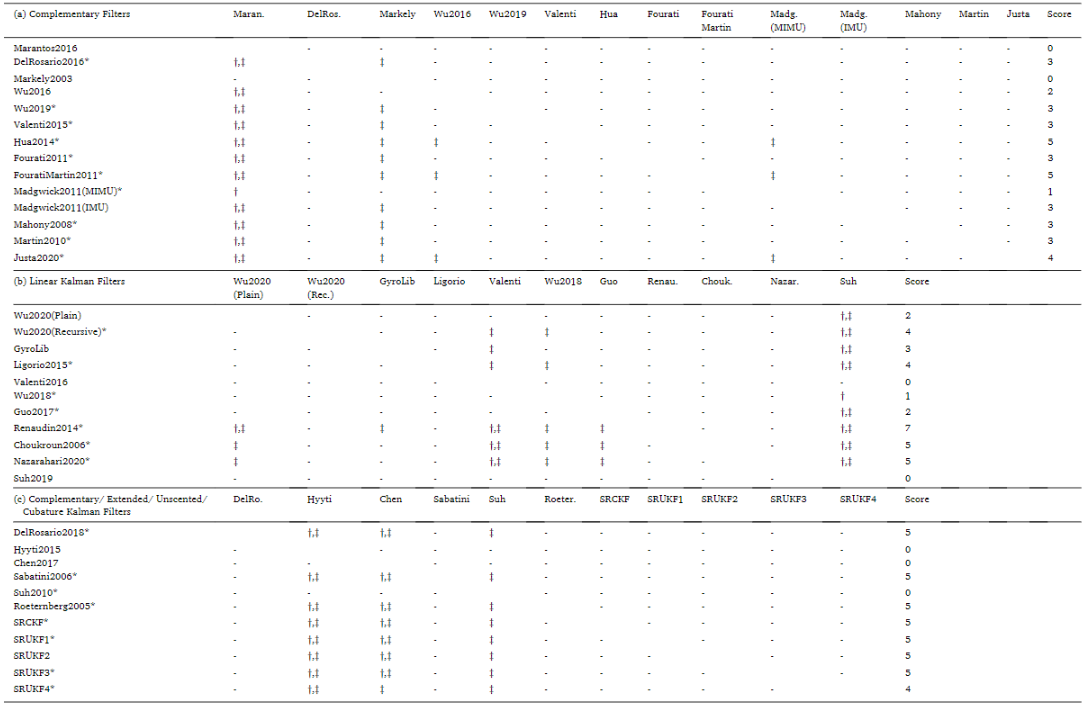
\includegraphics[width=1.2\textwidth]{full_comp.PNG}
\end{figure}

\begin{figure}[!h]
  \caption{Comparison of a selection of Complimentary and Kalman filters with different MIMUs [1]}
  \centering
  \label{fig:inputcomp}
  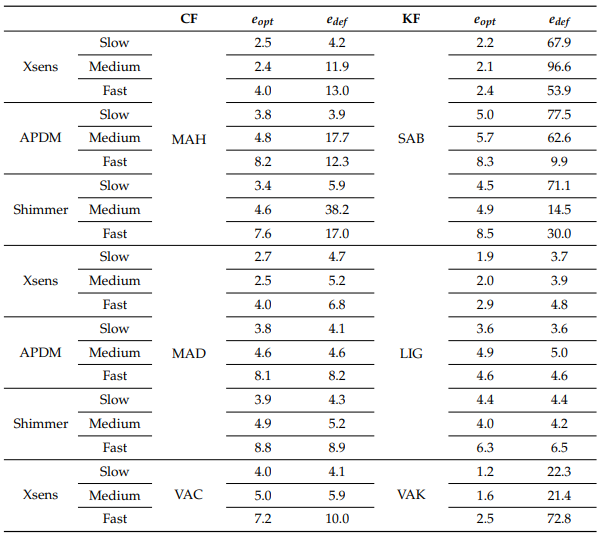
\includegraphics[width=1\textwidth]{input_comp.PNG}
\end{figure}
\newpage
\begin{figure}[!h]
  \caption{Continuation of figure \ref{fig:inputcomp}[1]}
  \centering
  \label{fig:inputcomp2}
  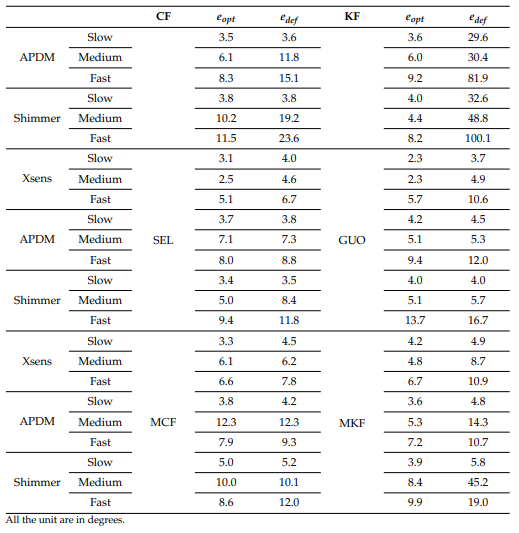
\includegraphics[width=1\textwidth]{input_comp2.PNG}
\end{figure}
\newpage
\newpage
\newpage
\newpage
\newpage
\newpage
\clearpage
\subsection*{Bibliography}
[1] \textbf{Provided a source of comparison and motivates the selection of algorithms based on context}\newline
Caruso, M., Sabatini, A. M., Laidig, D., Seel, T., Knaflitz, M., Della Croce, U., \& Cereatti, A. (2021). Analysis of the Accuracy of Ten Algorithms for Orientation Estimation Using Inertial and Magnetic Sensing under Optimal Conditions: One Size Does Not Fit All. Sensors (Basel, Switzerland), 21(7), 2543. https://doi.org/10.3390/s21072543 \newline
[2] \textbf{Provided a source of comparison with a large range of methods and discusses standardising tuning methods and the need for them} \newline
Nazarahari, M., \& Rouhani, H. (2021). Sensor fusion algorithms for orientation tracking via magnetic and inertial measurement units: An experimental comparison survey. Information Fusion, 76, 8–23. https://doi.org/https://doi.org/10.1016/j.inffus.2021.04.009\newline
[3] \textbf{Provided a source of comparison for the different classes of sensor fusion algorithms specifically with regard to their use in human orientation estimation} \newline
Bergamini, E., Ligorio, G., Summa, A., Vannozzi, G., Cappozzo, A., \& Sabatini, A. (2014). Estimating Orientation Using Magnetic and Inertial Sensors and Different Sensor Fusion Approaches: Accuracy Assessment in Manual and Locomotion Tasks. Sensors (Basel, Switzerland), 14, 18625–18649. https://doi.org/10.3390/s141018625\newline
[4] \textbf{Provided an overview of the characteristics of MEMS sensors and their measurement properties regarding noise and bias among others} \newline
Woodman, O. J. (2007, August). An introduction to inertial navigation. Department of Computer Science and Technology |. 
https://www.cl.cam.ac.uk/techreports/UCAM-CL-TR-696.pdf\newline
[5] \textbf{Provided an overview of the state of MEMS sensors and the future of the measurement technology related to orientation estimation} \newline
Passaro, V., Cuccovillo, A., Vaiani, L., Carlo, M., \& Campanella, C. E. (2017). Gyroscope Technology and Applications: A Review in the Industrial Perspective. Sensors (Basel, Switzerland), 17(10), 2284. https://doi.org/10.3390/s17102284\newline
[6]\textbf{Provided an explanation of the pros and cons of quaternions as well as discussed reconvergence in sensor fusion algorithms} \newline
 Kok, M., \& Schön, T. B. (2019). A Fast and Robust Algorithm for Orientation Estimation Using Inertial Sensors. IEEE Signal Processing Letters, 26(11), 1673–1677. https://doi.org/10.1109/LSP.2019.2943995\newline
[7]\textbf{Provided a discussion about magnetic interference and how to compensate for it} \newline
 Zhu, M., Ouyang, W., \& Wu, Y. (2021). Orientation Estimation by Partial-State Updating Kalman Filter and Vectorial Magnetic Interference Detection. IEEE Transactions on Aerospace and Electronic Systems, 57(3), 1815–1826. https://doi.org/10.1109/TAES.2021.3050657\newline
[8] \textbf{Provided a discussion of motion models for filters as well as standstill detection} \newline
Gabriel, D., Baumgärtner, D., \& Görges, D. (2022). Accurate and robust state estimation for bicycles. Vehicle System Dynamics, 1–14. https://doi.org/10.1080/00423114.2022.2109491\newline
[9] \textbf{Provided an in depth explanation of complementary filters} \newline
Szczęsna, A., Pruszowski, P., Słupik, J., Pęszor, D., \& Polanski, A. (2015, October). Evaluation of Improvement in Orientation Estimation Through the Use of the Linear Acceleration Estimation in the Body Model. https://doi.org/10.1007/978-3-319-23437-3\_32\newline
[10] \textbf{Provided an overview of the concepts that are neeeded to understand contemporay state estimation techniques} \newline
Bai, L. (2022). 3D orientation estimation using inertial sensors. Journal of Electrical Technology UMY, 6(1), 12–21. https://doi.org/10.18196/jet.v6i1.14638 \newline
[11] \textbf{Provided a source of discussion regarding the application of orientation estimation to vehicles as well as the multibin method of orientation estimation} \newline
Tu, H., Peng, S., Leung, V., \& Gao, R. (2021). SoK: Vehicle Orientation Representations for Deep Rotation Estimation.\newline
[12] \textbf{Influence of temperature on orientation estimation} \newline
Bereska, D., Daniec, K., Ilewicz, W., Jędrasiak, K., Koteras, R., Nawrat, A., \& Pacholczyk, M. (2016). Influence of temperature on measurements of 3-axial accelerometers and gyroscopes: Embedded into inertial measurement unit. 2016 International Conference on Signals and Electronic Systems (ICSES), 200–205. https://doi.org/10.1109/ICSES.2016.7593851\newline
[13] \textbf{The Justa2020 Complementary filter} \newline
Justa, J., Šmídl, V., \& Hamáček, A. (2020). Fast AHRS Filter for Accelerometer, Magnetometer, and Gyroscope Combination with Separated Sensor Corrections. Sensors, 20(14). https://doi.org/10.3390/s20143824\newline
[14] \textbf{The Hua2014 Complementary filter} \newline
Hua, M.D., Ducard, G., Hamel, T., Mahony, R. and Rudin, K., 2013. Implementation of a nonlinear attitude estimator for aerial robotic vehicles. IEEE Transactions on Control Systems Technology, 22(1), pp.201-213.
[15] \textbf{The Sabatini2006 Extended Kalman Filter} \newline
Sabatini, A.M., 2006. Quaternion-based extended Kalman filter for determining orientation by inertial and magnetic sensing. IEEE transactions on Biomedical Engineering, 53(7), pp.1346-1356.\newline
[16] \textbf{The Madgwick Complementary filter}\newline
Madgwick, S.O., Harrison, A.J. and Vaidyanathan, R., 2011, June. Estimation of IMU and MARG orientation using a gradient descent algorithm. In 2011 IEEE international conference on rehabilitation robotics (pp. 1-7). IEEE.\newline
[17] \textbf{Comparison of EKF and UKFs}\newline
Yang, C., Shi, W., \& Chen, W. (2017). Comparison of Unscented and Extended Kalman Filters with Application in Vehicle Navigation. Journal of Navigation, 70(2), 411-431. doi:10.1017/S0373463316000655\newline
[18] \textbf{Comparison of particle filters to Kalman filters}\newline
Konatowski, S., Kaniewski, P., \& Matuszewski, J. (2016). Comparison of Estimation Accuracy of EKF, UKF and PF Filters. Annual of Navigation, 23. https://doi.org/10.1515/aon-2016-0005\newline
[19] \textbf{The Renaudin2014 Linear Kalman Filter}\newline
Renaudin, V. and Combettes, C., 2014. Magnetic, acceleration fields and gyroscope quaternion (MAGYQ)-based attitude estimation with smartphone sensors for indoor pedestrian navigation. Sensors, 14(12), pp.22864-22890.\newline
[20] \textbf{IMU market growth projection}\newline
Inertial measurement unit [IMU] market size | global report 2029. (n.d.). Fortune Business Insights™ | Global Market Research Reports \& Consulting.
https://www.fortunebusinessinsights.com/industry-reports/inertial-measurement-unit-market-101827
\end{document}
